% Provenance (never printed): the comparative-advantage strand of ../economics_series.md (grade 7; "Ricardo with real
% weight": the result is named once here, the model is owned by Book 2 g10). Brief: sources/book1/BRIEFS.md, g7-03.
% Chart data: figdata/grade-7/03-comparative-advantage (WDI NE.EXP.GNFS.ZS, SP.POP.TOTL; Brenland/Kestria ricardo.csv).
% Ledger: g7:japan-opening-1859, g7:bernhofen-brown-2004, g7:japan-exports-silk-tea, g7:japan-imports-textiles.
\chapter{Gains from Trade: Comparative Advantage}\label{ch:g7:comparative-advantage}

\begin{openingchart}{Exports of goods and services as a share of output and
population, in 2024, one dot per country; population on a times-ten
scale.}{World Bank, World Development Indicators, NE.EXP.GNFS.ZS and SP.POP.TOTL,
2024}
\begin{tikzpicture}
\begin{semilogxaxis}[omincomex, xmin=0.005, xmax=3000, ymin=0, ymax=200,
  xtickten={-3,...,9}, xlabel={Population (millions, times-ten scale)},
  ylabel={Exports, percent of output}]
\addplot table[x=pop, y=exports]
  {figdata/grade-7/03-comparative-advantage/out/exports_size.csv};
\end{semilogxaxis}
\end{tikzpicture}
\end{openingchart}

% figdata: exports_pairs (USA 340.0 11.0; CHN 1408.98 20.4; IND 1450.94 22.1; NLD 17.99 82.5; IRL 5.4 144.0;
% LUX 0.68 191.5; BEL 11.86 79.3)
% figdata: facts (large_n 15, large_median 21.9, small_n 40, small_median 49.25)
Small countries sell a large part of what they produce abroad. In 2024, the \omterm{def:g6:a-connected-world:export}{exports}
of the Netherlands, with 18 million people, were worth $82.5\,\%$ of its output; those
of Luxembourg, with fewer than a million, $191.5\,\%$ (the reason a share can pass
$100\,\%$ was given in \cref{ch:g6:a-connected-world}). The United States, with 340
million people, exported $11.0\,\%$ of its output; India, $22.1\,\%$. Among the 15
countries of more than 100 million people, the middle value was $21.9\,\%$; among the
40 countries of fewer than 2 million, about $49\,\%$.

A small country cannot make everything well: it makes a few things and buys the rest.
But why would a country, or a person, buy from others what it could make itself, even
make faster? This chapter gives the answer: trade pays whenever two sides give up
different amounts to make the same things.

\begin{recall}
The \omterm{def:g7:scarcity-and-opportunity-cost:opportunity-cost}{opportunity cost} of a choice is the value of the best option given up
(\cref{ch:g7:scarcity-and-opportunity-cost}). \omterm{def:g7:specialisation:specialisation}{Specialisation} and exchange were defined
in \cref{ch:g7:specialisation}.
\end{recall}

\begin{omfigure}
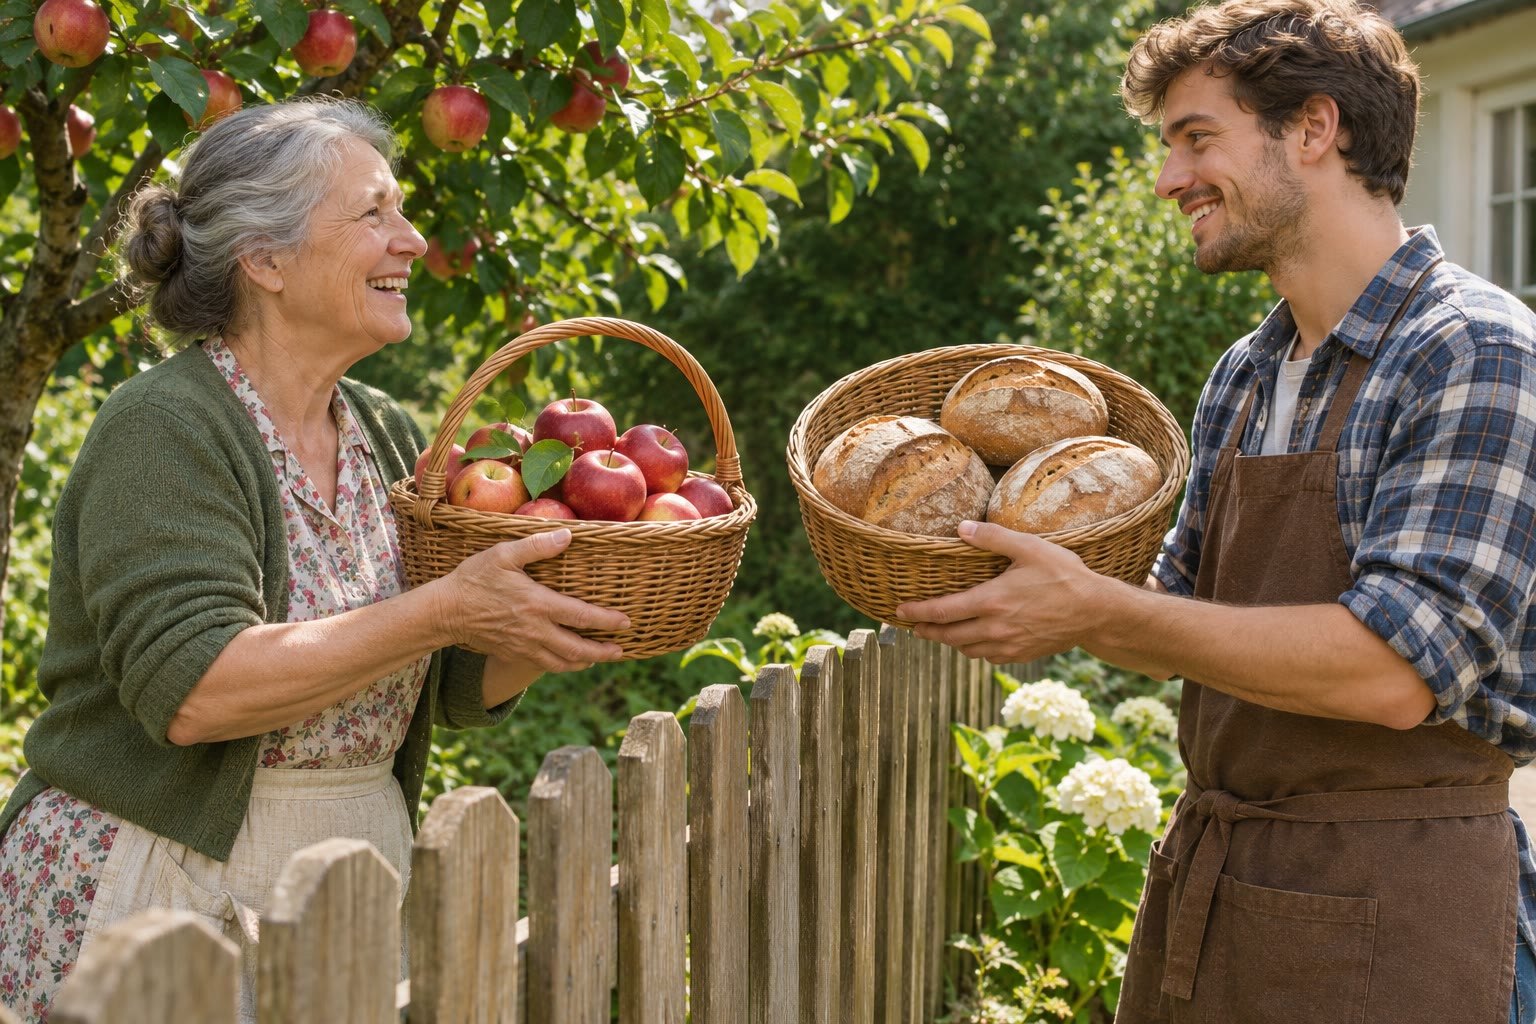
\includegraphics[width=0.55\linewidth]{images/book1/ai/g7-comparative-advantage-neighbours.jpg}

{\small Two neighbours swap apples for bread. Each gives what costs her or him less to
make.}
\end{omfigure}

\section{Two people, two tasks, a table of hours}

Nadia and Omar are invented neighbours. Each can bake bread and sew shirts, and each
has 24 hours a week for this work. The table gives the hours each needs for one unit.

\begin{center}
\begin{tabular}{lcc}
\toprule
 & One loaf & One shirt \\
\midrule
Nadia & 1 hour & 3 hours \\
Omar  & 2 hours & 4 hours \\
\bottomrule
\end{tabular}
\end{center}

\begin{measure}[Hours per unit]
A table of hours per unit is the simplest way to describe what a person, a region or a
country can produce. Each number is a count of the work needed for one unit, with the
tools, land and skills the producer has. A lower number means a more productive
producer. For whole countries, economists measure output per hour by industry, and the
comparison is the same.
\end{measure}

\begin{omfigure}
\begin{tikzpicture}[econ, x=1cm, y=0.55cm]
  \foreach \y/\name in {3/Nadia, 0.5/Omar} \node[anchor=east, font=\footnotesize] at (-0.2,\y) {\name};
  % Nadia: loaf 1 h, shirt 3 h; Omar: loaf 2 h, shirt 4 h (1 cm per hour)
  \fill[omMeth!45] (0,3.4) rectangle (1,4.2);   \node[right, font=\scriptsize] at (1,3.8) {loaf: 1 h};
  \fill[omDef!40]  (0,2.0) rectangle (3,2.8);   \node[right, font=\scriptsize] at (3,2.4) {shirt: 3 h};
  \fill[omMeth!45] (0,0.9) rectangle (2,1.7);   \node[right, font=\scriptsize] at (2,1.3) {loaf: 2 h};
  \fill[omDef!40]  (0,-0.5) rectangle (4,0.3);  \node[right, font=\scriptsize] at (4,-0.1) {shirt: 4 h};
  \draw[-{Stealth}] (0,-1) -- (5.6,-1) node[right, font=\scriptsize] {hours};
  \foreach \x in {0,...,5} \draw (\x,-1) -- (\x,-1.2) node[below, font=\scriptsize] {\x};
\end{tikzpicture}

{\small The hours that Nadia and Omar need for one loaf and one shirt. Nadia's bars are
shorter for both goods.}
\end{omfigure}

\section{Absolute advantage}

\begin{definition}[Absolute advantage]\label{def:g7:comparative-advantage:absolute-advantage}
A producer has an \emph{absolute advantage}\index{absolute advantage} in a good when it
needs fewer hours (or less of any input) than another producer to make one unit of it.
\end{definition}

Nadia has an \omterm{def:g7:comparative-advantage:absolute-advantage}{absolute advantage} in both goods: one hour against two for a loaf, three
against four for a shirt. One might think that she gains nothing by trading with Omar.
The next section shows that she does.

\section{Comparative advantage}

The three hours that Nadia spends on a shirt could make three loaves: her \omterm{def:g7:scarcity-and-opportunity-cost:opportunity-cost}{opportunity
cost} of a shirt is 3 loaves. Omar's four hours for a shirt could make two loaves: his
\omterm{def:g7:scarcity-and-opportunity-cost:opportunity-cost}{opportunity cost} of a shirt is 2 loaves. The other way round, a loaf costs Nadia
$\tfrac13$ of a shirt and Omar $\tfrac12$ of a shirt.

\begin{center}
\begin{tabular}{lcc}
\toprule
\omterm{def:g7:scarcity-and-opportunity-cost:opportunity-cost}{Opportunity cost} & of one loaf & of one shirt \\
\midrule
Nadia & $\tfrac13$ shirt & 3 loaves \\
Omar  & $\tfrac12$ shirt & 2 loaves \\
\bottomrule
\end{tabular}
\end{center}

\begin{definition}[Comparative advantage]\label{def:g7:comparative-advantage:comparative-advantage}
A producer has a \emph{comparative advantage}\index{comparative advantage} in a good
when its \omterm{def:g7:scarcity-and-opportunity-cost:opportunity-cost}{opportunity cost} of producing that good is lower than another producer's.
\end{definition}

Nadia has the \omterm{def:g7:comparative-advantage:comparative-advantage}{comparative advantage} in bread ($\tfrac13$ of a shirt against $\tfrac12$),
and Omar in shirts (2 loaves against 3). Omar is slower at everything, yet a shirt
costs him fewer loaves than it costs Nadia. Every producer has a \omterm{def:g7:comparative-advantage:comparative-advantage}{comparative advantage}
in something, unless the two \omterm{def:g7:scarcity-and-opportunity-cost:opportunity-cost}{opportunity costs} are exactly equal. This result,
which economists owe to David Ricardo, is the reason trade can benefit both sides.

\section{Both gain: the exchange ratios that work}

\begin{example}
\emph{Without trade}, each spends half of the week on each good. Nadia makes $12 \div
1 = 12$ loaves and $12 \div 3 = 4$ shirts; Omar makes $12 \div 2 = 6$ loaves and $12
\div 4 = 3$ shirts. Together: 18 loaves and 7 shirts.

\emph{With \omterm{def:g7:specialisation:specialisation}{specialisation}}, Omar sews all week: $24 \div 4 = 6$ shirts. Nadia sews one
shirt (3 hours) and bakes for the other 21 hours: 21 loaves. Together: 21 loaves and 7
shirts. The same shirts, and 3 more loaves, from the same hours.

\emph{With trade}, Omar gives Nadia 3 shirts for $7.5$ loaves, that is $2.5$ loaves per
shirt. Omar ends with 3 shirts and $7.5$ loaves (before: 3 and 6). Nadia ends with $1 +
3 = 4$ shirts and $21 - 7.5 = 13.5$ loaves (before: 4 and 12). Each has $1.5$ loaves
more than without trade.
\end{example}

\begin{definition}[Gains from trade]\label{def:g7:comparative-advantage:gains-from-trade}
The \emph{gains from trade}\index{gains from trade} are the extra goods that the two
sides can consume when they specialise and exchange, compared with producing everything
for themselves.
\end{definition}

\begin{definition}[Exchange ratio]\label{def:g7:comparative-advantage:exchange-ratio}
An \emph{exchange ratio}\index{exchange ratio} is the quantity of one good given for one
unit of another in an exchange: for example, $2.5$ loaves per shirt.
\end{definition}

Not every \omterm{def:g7:comparative-advantage:exchange-ratio}{exchange ratio} works. Omar will not sell a shirt for fewer than 2 loaves: he
could bake 2 loaves himself with the hours of a shirt. Nadia will not pay more than 3
loaves for a shirt: she could sew it herself for 3 loaves. Any ratio between 2 and 3
loaves per shirt gives both of them a gain. Where the ratio falls inside that range
decides how the gain is shared.

\begin{omfigure}
\begin{tikzpicture}[econ, x=3cm, y=1cm]
  \fill[omMeth!25] (2,-0.2) rectangle (3,0.2);
  \draw[-{Stealth}] (0.8,0) -- (3.9,0) node[right, font=\scriptsize] {loaves per shirt};
  \foreach \x in {1,1.5,2,2.5,3,3.5} \draw (\x,-0.1) -- (\x,0.1) node[pos=0, below=1pt, font=\scriptsize] {\x};
  \draw[thick] (2,-0.25) -- (2,0.25); \draw[thick] (3,-0.25) -- (3,0.25);
  \fill (2.5,0) circle (2pt);
  \node[above, font=\scriptsize] at (2.5,0.25) {both gain};
  \node[above, font=\scriptsize] at (1.4,0.25) {Omar refuses};
  \node[above, font=\scriptsize] at (3.45,0.25) {Nadia refuses};
  \node[font=\scriptsize, align=center] at (2,-1.05) {Omar's\\opportunity cost\\of a shirt};
  \node[font=\scriptsize, align=center] at (3,-1.05) {Nadia's\\opportunity cost\\of a shirt};
\end{tikzpicture}

{\small The \omterm{def:g7:comparative-advantage:exchange-ratio}{exchange ratios} at which both Nadia and Omar gain lie between their two
\omterm{def:g7:scarcity-and-opportunity-cost:opportunity-cost}{opportunity costs} of a shirt. The dot is the ratio of the example.}
\end{omfigure}

\begin{model}{Comparative advantage, two people and two goods}
\assumes Two producers, two goods; each unit takes a fixed number of hours; each
producer has a fixed number of hours; exchange is free and costs nothing.
\predicts Each producer \omterm{def:g7:specialisation:specialisation}{specialises} in the good of its lower \omterm{def:g7:scarcity-and-opportunity-cost:opportunity-cost}{opportunity cost}; at any
\omterm{def:g7:comparative-advantage:exchange-ratio}{exchange ratio} between the two \omterm{def:g7:scarcity-and-opportunity-cost:opportunity-cost}{opportunity costs}, both consume more than without trade.
\tested Japan's opening to trade after 1859 (the box below). The opening chart, where
small countries trade a larger share of their output, is consistent with the model but
does not test it: country size alone would give the same picture.
\breaks Moving from one task to another costs time; carrying goods costs money, which
narrows or closes the range of ratios; inside a country, the gains are not shared by
everyone, which the grades 10--12 volume takes up.
\end{model}

\begin{record}[Japan opens to trade]
% ledger: g7:japan-opening-1859, g7:bernhofen-brown-2004, g7:japan-exports-silk-tea, g7:japan-imports-textiles
For more than two centuries, Japan traded almost nothing with the rest of the world.
In July 1859, under pressure from Western powers, its ports opened to foreign trade,
suddenly and with low taxes on \omterm{def:g6:a-connected-world:import}{imports} and \omterm{def:g6:a-connected-world:export}{exports}. Prices inside Japan, which had
been set by Japanese costs alone, could now be compared with world prices. Japan began
to \omterm{def:g6:a-connected-world:export}{export} the goods that were cheap at home compared with abroad --- silk, silkworm eggs
and tea made about 80\,\% of its \omterm{def:g6:a-connected-world:export}{exports} from 1868 to 1875 --- and to \omterm{def:g6:a-connected-world:import}{import} those that
were dear at home: about half of its \omterm{def:g6:a-connected-world:import}{imports} were cotton and woollen cloth. A study of
these years valued each year's trade, good by good, at the prices Japan had before the
opening. Taken together, Japan's \omterm{def:g6:a-connected-world:export}{exports} were goods that had been cheap at home and its
\omterm{def:g6:a-connected-world:import}{imports} goods that had been dear, in every year from 1868 to 1875, as the
comparative-advantage model predicts (Bernhofen and Brown, 2004).
\end{record}

\section{Two regions}

The same reasoning works for regions and countries. The series' two invented countries,
Brenland and Kestria, both grow grain and weave cloth. The chart gives the hours of work
each needs for one unit.

\begin{omchart}{Hours of work needed for one unit of grain and one unit of cloth, in
Brenland and in Kestria (invented data).}{The series' invented countries, Brenland and
Kestria}
\begin{tikzpicture}
\begin{axis}[omrecord, ybar, bar width=18pt, ymin=0, ymax=14, grid=none, ymajorgrids,
  enlarge x limits=0.5, xtick=data, xticklabels={Grain, Cloth}, symbolic x coords={grain, cloth},
  ylabel={Hours per unit}, nodes near coords, every node near coord/.append style={font=\scriptsize},
  legend style={at={(0.5,-0.15)}, anchor=north, legend columns=2}, height=0.42\linewidth]
\addplot[fill=omMeth!55, draw=omMeth] table[x=good, y=brenland]
  {figdata/grade-7/03-comparative-advantage/out/ricardo.csv};
\addplot[fill=omExo!45, draw=omExo] table[x=good, y=kestria]
  {figdata/grade-7/03-comparative-advantage/out/ricardo.csv};
\legend{Brenland, Kestria}
\end{axis}
\end{tikzpicture}
\end{omchart}

% figdata: ricardo (grain: brenland 2, kestria 12; cloth: brenland 4, kestria 6)
% figdata: facts (brenland_cloth_in_grain 2, kestria_cloth_in_grain 0.5)
Brenland needs fewer hours for both goods: it has the \omterm{def:g7:comparative-advantage:absolute-advantage}{absolute advantage} in grain and in
cloth. But a unit of cloth costs Brenland $4 \div 2 = 2$ units of grain, and Kestria only
$6 \div 12 = 0.5$ unit of grain. Kestria has the \omterm{def:g7:comparative-advantage:comparative-advantage}{comparative advantage} in cloth, and
Brenland in grain. Both countries gain if Brenland sends grain to Kestria and Kestria
sends cloth to Brenland, at any \omterm{def:g7:comparative-advantage:exchange-ratio}{exchange ratio} between $0.5$ and 2 units of grain per
unit of cloth.

\section{Exercises}

\begin{exercise}[$\star$]\label{exo:g7:comparative-advantage:1}
Pia needs 2 hours to bake a cake and 3 hours to knit a scarf. Leo needs 1 hour for a cake
and 4 hours for a scarf. Who is faster at each task?
\end{exercise}

\begin{exercise}[$\star$]\label{exo:g7:comparative-advantage:2}
Sara bakes a loaf in 1 hour and sews a shirt in 4 hours. What is her \omterm{def:g7:scarcity-and-opportunity-cost:opportunity-cost}{opportunity cost} of
one shirt, in loaves?
\end{exercise}

\begin{exercise}[$\star$]\label{exo:g7:comparative-advantage:3}
Use the values in the text. What share of its output did the Netherlands \omterm{def:g6:a-connected-world:export}{export} in 2024,
and the United States? Which country has the larger population?
\end{exercise}

\begin{exercise}[$\star$]\label{exo:g7:comparative-advantage:4}
Two invented regions make cars and rice. The North needs 50 hours for a car and 20 hours
for a tonne of rice; the South needs 80 hours for a car and 10 hours for a tonne of rice.
Which region has the \omterm{def:g7:comparative-advantage:absolute-advantage}{absolute advantage} in each good?
\end{exercise}

\begin{exercise}[$\star\star$]\label{exo:g7:comparative-advantage:5}
Use the regions of exercise 4. (a) Compute each region's \omterm{def:g7:scarcity-and-opportunity-cost:opportunity-cost}{opportunity cost} of one car, in
tonnes of rice. (b) Which region has the \omterm{def:g7:comparative-advantage:comparative-advantage}{comparative advantage} in cars, and which in
rice?
\end{exercise}

\begin{exercise}[$\star\star$]\label{exo:g7:comparative-advantage:6}
Ana bakes a loaf in 1 hour and makes a chair in 5 hours; Bo bakes a loaf in 2 hours and
makes a chair in 5 hours. Each works 20 hours. (a) If each spends half of the time on each
good, how many loaves and chairs do they make together? (b) Who has the \omterm{def:g7:comparative-advantage:comparative-advantage}{comparative
advantage} in chairs? (c) If each \omterm{def:g7:specialisation:specialisation}{specialises} fully in the good of his or her \omterm{def:g7:comparative-advantage:comparative-advantage}{comparative
advantage}, what do they make together? What is gained?
\end{exercise}

\begin{exercise}[$\star\star$]\label{exo:g7:comparative-advantage:7}
In the example of Nadia and Omar, Omar gives 3 shirts at a ratio of $2.2$ loaves per
shirt instead of $2.5$. (a) How many loaves does Omar get? (b) Compute the gain of each
compared with no trade. (c) Who gains more than at $2.5$?
\end{exercise}

\begin{exercise}[$\star\star$]\label{exo:g7:comparative-advantage:8}
Nadia offers Omar $1.5$ loaves per shirt. (a) Would Omar accept? Explain with his
\omterm{def:g7:scarcity-and-opportunity-cost:opportunity-cost}{opportunity cost}. (b) What happens to the \omterm{def:g7:comparative-advantage:gains-from-trade}{gains from trade}?
\end{exercise}

\begin{exercise}[$\star\star$]\label{exo:g7:comparative-advantage:9}
What observation about a country's trade would contradict the model ``\omterm{def:g7:comparative-advantage:comparative-advantage}{Comparative
advantage}, two people and two goods''? Describe it.
\end{exercise}

\begin{exercise}[$\star\star\star$]\label{exo:g7:comparative-advantage:10}
Use the chart of Brenland and Kestria. (a) Give each country's \omterm{def:g7:scarcity-and-opportunity-cost:opportunity-cost}{opportunity cost} of one unit
of grain, in units of cloth. (b) They trade at 1 unit of grain for 1 unit of cloth.
Brenland gives 1 unit of grain: how many hours of work did it cost Brenland, and how many
hours would Brenland have needed to weave the unit of cloth it gets? (c) Do the same
for Kestria, which gives 1 unit of cloth. (d) Who saves hours?
\end{exercise}

\begin{exercise}[$\star\star\star$]\label{exo:g7:comparative-advantage:11}
Nadia becomes twice as fast at both tasks: half an hour per loaf, $1.5$ hours per shirt.
(a) Compute her new \omterm{def:g7:scarcity-and-opportunity-cost:opportunity-cost}{opportunity cost} of a shirt. (b) Does trade with Omar still pay for
both? (c) If instead Nadia became faster only at shirts, needing 2 hours for one, what
would happen to the \omterm{def:g7:comparative-advantage:gains-from-trade}{gains from trade}?
\end{exercise}

\begin{exercise}[$\star\star\star$]\label{exo:g7:comparative-advantage:12}
When Brenland \omterm{def:g6:a-connected-world:import}{imports} Kestria's cloth, some of Brenland's weavers lose customers.
(a) Does the model of the chapter say that everyone in Brenland gains? (b) What does the
model leave out? (c) What data would show who in Brenland gains and who loses?
\end{exercise}

\section{Problem: Grain and Cloth across the Border}

\begin{problem}[{Weekend problem --- Brenland and Kestria's hours per unit,
opportunity costs and specialisation, and each country's gain from trading}]
\label{pb:g7:comparative-advantage:1}
Brenland and Kestria are the series' invented countries; the hours per unit are those of
the chart above. Each country has 120 million hours of work a year for grain and cloth.
Quantities are in millions of units.

\medskip
\noindent\textbf{Part I --- Hours per unit.}
\begin{enumerate}
  \item Write the table of hours per unit of grain and of cloth for the two countries.
  \item Which country has the \omterm{def:g7:comparative-advantage:absolute-advantage}{absolute advantage} in grain, and which in cloth?
  \item Without trade, each country spends half of its hours on each good. How much grain
        and cloth does each country produce?
  \item How much grain and cloth do the two countries produce together?
\end{enumerate}

\medskip
\noindent\textbf{Part II --- Opportunity costs and specialisation.}
\begin{enumerate}[resume]
  \item Compute each country's \omterm{def:g7:scarcity-and-opportunity-cost:opportunity-cost}{opportunity cost} of one unit of cloth, in grain.
  \item Compute each country's \omterm{def:g7:scarcity-and-opportunity-cost:opportunity-cost}{opportunity cost} of one unit of grain, in cloth.
  \item Which country has the \omterm{def:g7:comparative-advantage:comparative-advantage}{comparative advantage} in each good?
  \item Kestria weaves cloth with all its hours. Brenland weaves 5 million units of cloth
        and grows grain with the rest of its hours. Compute the production of each country
        and the total. Compare with question 4.
\end{enumerate}

\medskip
\noindent\textbf{Part III --- Trade.} Kestria sends 10 million units of cloth to Brenland
and receives 10 million units of grain: 1 unit of grain per unit of cloth.
\begin{enumerate}[resume]
  \item What does Kestria have to consume after trade?
  \item What does Brenland have to consume after trade?
  \item Compare with Part I: what is each country's gain, in units of grain?
  \item Check that the two gains add up to the extra production found in question 8.
  \item At a ratio of $1.5$ units of grain per unit of cloth (Kestria still sends 10 million
        units of cloth), compute each country's gain in grain. Who gains more now?
\end{enumerate}
\end{problem}
